% 两轮足机器人跳跃控制: SRL+VMC方法与组件消融
% 编译: latexmk -xelatex main.tex

% ==================== 武汉科技大学研究生小论文格式 ====================
\documentclass[12pt,a4paper,fontset=fandol]{ctexart}

% ---------- 页面设置 ----------
\usepackage[top=2.5cm, bottom=2.5cm, left=2.5cm, right=2.5cm]{geometry}
\usepackage{setspace}
\setstretch{1.25}
\usepackage{fancyhdr}
\pagestyle{fancy}
\fancyhf{}
\fancyhead[C]{\zihao{-5} 武汉科技大学研究生小论文}
\fancyfoot[C]{\thepage}
\renewcommand{\headrulewidth}{0.4pt}

% ---------- 基础宏包 ----------
\usepackage{amsmath, amssymb, amsthm, bm}
\usepackage{graphicx}
\usepackage{subcaption}
\usepackage{booktabs, array}
\usepackage{algorithm}
\usepackage{algpseudocode}
\floatname{algorithm}{算法}
\usepackage[colorlinks=true,linkcolor=black,citecolor=black,urlcolor=blue]{hyperref}
\usepackage[backend=biber,style=gb7714-2015,sorting=none]{biblatex}
\addbibresource{data/ref.bib}
\usepackage{caption}
\usepackage{enumitem}
\usepackage{textcomp}
\usepackage{tabularx}

% ---------- 图表标题格式 ----------
\captionsetup{font={small,bf},labelfont={small,bf},labelsep=space}
\setlength{\textfloatsep}{8pt}
\setlength{\floatsep}{8pt}
\setlength{\intextsep}{6pt}

% ---------- 编号设置 ----------
\numberwithin{equation}{section}
\numberwithin{figure}{section}
\numberwithin{table}{section}
\renewcommand{\theequation}{\arabic{section}.\arabic{equation}}
\renewcommand{\thefigure}{\arabic{section}.\arabic{figure}}
\renewcommand{\thetable}{\arabic{section}.\arabic{table}}

% ---------- 列表格式 ----------
\setlist{nosep, leftmargin=2em}

% ---------- 数学环境 ----------
\newtheorem{theorem}{定理}

% ---------- 图片路径 ----------
\graphicspath{{../../picture/paper/jump/training/2x2/v3/}{../../picture/paper/jump/final_perf/2x1/v3/}{../../picture/paper/jump/traj/2x1/v3/}{figures/}}

% ==================== 论文信息 ====================
\title{\heiti\zihao{3} 融合SLIP-FSM结构先验与虚拟模型控制的\\两轮足机器人强化学习跳跃方法}

\author{
    \zihao{4}
    肖琦$^{1}$\quad 汤勃$^{1}$\quad 孙伟$^{1}$ \\
    {\zihao{-5} (1. 武汉科技大学 机械工程学院，湖北 武汉 430081)}
}
\date{}

\begin{document}

\maketitle
\thispagestyle{fancy}

% ---------- 中文摘要 ----------
\begin{abstract}
\noindent\textbf{摘要：}两轮足机器人的跳跃同时涉及非线性腿部蹬伸、轮地滚动约束与落地冲击，单纯依赖模型前馈难以适应动力学误差，而无结构先验的强化学习又易收敛到“不下蹲”或“小幅离地”等局部最优。为此，本文提出一种SRL+VMC跳跃控制方法：以SLIP的储能—释能机理构造六状态相位有限状态机，生成虚拟腿长与轮速前馈参考；以PPO策略学习虚拟腿空间的残差修正；再由相位自适应VMC将虚拟力和力矩通过雅可比映射为关节力矩。针对策略在下蹲相提前上升导致的双重运动，进一步提出与FSM状态一致的蹬伸奖励门控。在MuJoCo中对xqrobotwl以1024个并行环境训练后，所得策略呈现“下蹲—蹬伸—腾空—落地—恢复”轨迹。20次独立评估的平均跳高为$0.308\pm0.006$\,m；20次连续触发测试中19次形成真实腾空、18次完成落地恢复，完整成功率为90\%。组件消融中，SRL+VMC的平均跳高高于SRL、PPO+VMC和纯PPO，说明相位结构先验、残差学习与虚拟腿力控具有互补作用。
\par\noindent\textbf{关键词：} 两轮足机器人；跳跃控制；强化学习；SLIP模型；虚拟模型控制；相位门控奖励
\end{abstract}

% ---------- 英文摘要 ----------
\begin{center}
{\large\bfseries Reinforcement-Learning Jumping for a Wheel-Legged Robot by Combining a SLIP-FSM Structural Prior with Virtual Model Control}

\vspace{0.3cm}
{\normalsize XIAO Qi$^{1}$, TANG Bo$^{1}$, SUN Wei$^{1}$}

{\small (1. School of Mechanical Engineering, Wuhan University of Science and Technology, Wuhan 430081, China)}
\end{center}

\begin{quote}
\noindent\textbf{Abstract:} Jumping a two-wheel-legged robot couples nonlinear leg extension, rolling contact and landing impact. Pure model-based feedforward control is sensitive to modeling errors, whereas reinforcement learning without structural priors readily converges to shallow or mistimed jumps. This paper proposes an SRL+VMC controller that combines three complementary elements. A six-state finite-state machine derived from the energy-storage and release mechanism of SLIP supplies phase-dependent virtual-leg and wheel-speed references; a PPO policy learns residual corrections in virtual-leg coordinates; and a phase-adaptive virtual model controller maps the desired virtual forces and torques to joint torques. We further gate thrust-related rewards by the physical FSM state to eliminate a double-motion failure in which the policy rises prematurely during crouching. After training with 1,024 parallel MuJoCo environments, the policy produces a crouch--thrust--flight--landing--recovery trajectory. Its mean jump height over 20 independent evaluations is $0.308\pm0.006$\,m. In a 20-attempt repeated-trigger test, 19 attempts become airborne and 18 complete landing recovery, yielding a 90\% overall success rate. A component ablation against SRL, PPO+VMC and PPO shows that the complete SRL+VMC controller yields the largest mean jump height, supporting the complementarity of phase priors, residual learning and virtual-leg force control.

\par\noindent\textbf{Keywords:} wheel-legged robot; jumping control; reinforcement learning; SLIP model; virtual model control; phase-gated reward
\end{quote}

\section{引言}

在搜救、仓储巡检与野外探测等非结构化环境中，机器人需要跨越沟壑、台阶等障碍，跳跃能力是完成这类任务的关键前提~\cite{mo2020jumping, koh2015jumping}。两轮足机器人（如Ascento~\cite{klemm2020ascento}、FLORES~\cite{song2025flores}）兼顾轮式平台的能效与腿式系统的越障能力，但其跳跃控制面临双足或四足平台不曾遭遇的独特难题：车轮以滚动方式与地面接触，落地阶段的轮地速度不匹配会直接引发滑移或倾倒，且机身俯仰与车轮转动之间存在强耦合，地面欠驱动约束贯穿整个跳跃过程。

机器人跳跃控制大体分为模型驱动与数据驱动两条路径。基于SLIP（Spring-Loaded Inverted Pendulum）模板模型~\cite{full1999templates, piovan2015reachability, piovan2016approximation}的方法以弹簧-质点系统刻画腿式运动“储能—释能”周期，生成的轨迹对多关节腿、滚动接触与地面扰动等真实因素缺乏应对~\cite{wensing2013slip}；模型预测控制~\cite{park2021cheetah, he2024cdm}虽能在线优化，但计算负担制约实时性。纯强化学习方法~\cite{kober2013rl, tao2024multiobjective, bellegarda2024robust}在跳远、跳高等动态任务中因缺乏物理先验而样本效率偏低，且时序性动作（先下蹲、再爆发、后缓冲）极易被策略用“代理量”偷懒钻空，收敛到不可控的局部最优。

近期混合框架将SLIP前馈与强化学习反馈结合，在双足、四足平台上取得了显著效果~\cite{hu2026srl}。然而该类方法多建立在点足接触上，未显式处理车轮在腾空和落地时的速度匹配，也没有回答结构化相位先验如何与轮腿机器人的虚拟腿力控协同。本文的出发点因此不是在关节PD与VMC之间做单纯二选一，而是建立一条“结构先验给出可执行时序—策略学习模型误差—VMC实现柔顺力控”的完整技术路线。

为此，本文提出\textbf{SRL+VMC}两轮足跳跃方法。该方法用SLIP-FSM提供下蹲、蹬伸、腾空、落地与恢复的相位结构，用PPO在虚拟腿空间中学习残差，并用相位自适应VMC完成力矩执行。纯PPO、PPO+VMC和SRL不再是论文的并列主角，而作为去除相位先验或VMC后的组件消融。主要贡献包括：
\begin{enumerate}[label=(\arabic*)]
    \item 提出融合SLIP-FSM、PPO残差学习与虚拟模型控制的SRL+VMC框架，将高层相位时序、中层策略适应和底层柔顺力控分层组合；
    \item 设计适用于轮腿跳跃的六状态参考与相位自适应VMC，在腾空和落地阶段显式引入轮速匹配，并在蹬伸和落地阶段切换刚度、阻尼与前馈力；
    \item 提出与物理FSM状态一致的蹬伸奖励门控，消除了下蹲相提前上升、回落后再次起跳的双重运动；
    \item 通过完整方法评估和2×2组件消融，定量分析结构先验与虚拟腿力控的互补性，并如实给出高跳与稳定落地之间的性能边界。
\end{enumerate}

\section{相关工作}

\subsection{基于SLIP模型的运动控制}

自Full和Koditschek~\cite{full1999templates}将SLIP确立为腿式运动模板以来，该模型在双足步态生成~\cite{geyer2019slip}、四足奔跑~\cite{he2024slip}与柔顺行走~\cite{xie2021vslip}等方向得到广泛验证，其可达性与近似控制亦有系统研究~\cite{piovan2015reachability, piovan2016approximation}。这些工作均不涉及车轮动力学——SLIP本质上是点足接触假设下的弹簧-质点系统，难以刻画滚动接触中的扭矩传递与速度匹配。本文沿用SLIP“储能—释能”的相位思想，但不仿真弹簧-质点动力学，而是将各跳跃阶段离散为有限状态机（FSM）的相位参考，以规避点足假设。

\subsection{轮腿机器人的跳跃控制}

在轮腿跳跃方面，Ascento~\cite{klemm2020ascento}利用运动基元配合LQR实现厘米级跳跃，ATRos~\cite{sun2025atros}在周期性跳跃中追求能效，Zeng等~\cite{zeng2026jumping}以NMPC优化轮腿跳跃轨迹，Patrizi等~\cite{patrizi2026rlmpc}用强化学习增强MPC。前者依赖手工调参、适应性有限，后者在线优化计算开销大，且这些方法均未将“控制层选择”与“参考轨迹必要性”作为可对照的设计维度。

\subsection{混合SLIP-RL框架与强化学习跳跃}

纯强化学习方法在四足跳跃~\cite{bellegarda2024robust}、双足跳跃优化~\cite{tao2024multiobjective}上取得进展，但样本效率与动作时序可学性仍是瓶颈。Hu等~\cite{hu2026srl}的SRL框架将SLIP前馈与PPO反馈结合，说明结构化动力学先验可以降低动态动作的学习难度。与其点足接触设定不同，本文将SLIP相位参考表达到虚拟腿空间，用VMC执行残差修正后的虚拟目标，并显式处理轮速匹配和落地恢复。PPO、PPO+VMC和SRL作为组件消融，用于检验完整SRL+VMC中两类结构元件的作用。

\section{本文方法}

\subsection{任务定义与SRL+VMC总体框架}

\textbf{任务。}机器人收到跳跃触发指令后，须依次完成\textbf{下蹲蓄力—爆发蹬伸—腾空—稳定落地—恢复站立}的完整周期。任务指令为
\begin{equation}
\bm{c}_t=[v_x,\,v_y,\,\omega_{\mathrm{yaw}},\,\theta_{\mathrm{tsk}},\,j_{\mathrm{cmd}}],
\end{equation}
其中$j_{\mathrm{cmd}}>0.5$时触发跳跃，触发关闭后要求机器人恢复稳定站立。

\textbf{方法框架。}SRL+VMC由三层组成（图~\ref{fig:framework}(a)）：SLIP-FSM在任务层输出相位$s_t$与虚拟腿前馈$u_{\mathrm{FSM}}$；PPO在策略层依据本体观测和相位学习残差$\Delta u_t$；VMC在执行层将融合后的虚拟腿目标映射为关节力矩。这种分层方式使策略无需从零探索跳跃时序，又能对前馈参考与真实动力学之间的偏差进行在线修正。

\textbf{组件消融。}为判断相位先验和VMC是否都有必要，在实验中沿“是否使用SLIP-FSM”与“是否使用VMC”构造四个变体（图~\ref{fig:framework}(b)、表~\ref{tab:design}）：
\begin{itemize}
    \item \textbf{控制空间}：关节空间位置控制——策略输出6维关节角偏移+2维轮速，经PD位置执行器映射为关节力矩；或VMC——策略输出虚拟腿坐标（腿角$\theta_0$、腿长$L_0$）、髋滚转角与轮速，经雅可比映射为关节力矩；
    \item \textbf{参考轨迹}：无参考——策略完全自学习跳跃时序；或SLIP-FSM相位参考——由六状态FSM提供每阶段的关节角/腿长参考，策略输出残差。
\end{itemize}

\begin{table}[htbp]
    \centering
    \caption{SRL+VMC的组件消融设计}
    \label{tab:design}
    \begin{tabular}{lcc}
        \toprule
        & 关节空间（位置控制） & 虚拟腿 VMC（力矩控制） \\
        \midrule
        无参考 & 纯PPO & PPO+VMC \\
        SLIP-FSM参考 & SRL & \textbf{SRL+VMC（本文）} \\
        \bottomrule
    \end{tabular}
\end{table}

其中，SRL去除VMC并使用关节位置PD，PPO+VMC去除SLIP-FSM相位先验，纯PPO同时去除两者。四个变体使用相同的PPO骨架、训练规模和跳跃任务；与控制表达相关的观测及奖励项随被测组件做必要适配，因此实验属于组件级消融，而非所有代码路径完全相同的严格因果实验。

\begin{figure}[htbp]
    \centering
    
\includegraphics[width=\columnwidth]{framework.pdf}
    \caption{SRL+VMC方法与消融关系：(a) SLIP-FSM相位先验、PPO残差策略和相位自适应VMC组成的分层控制链；(b) 通过去除相位先验或VMC得到的四个实验变体}
    \label{fig:framework}
\end{figure}

\subsection{机器人平台与仿真环境}

实验平台为两轮足机器人xqrobotwl（图~\ref{fig:robot}），质量参数来自CAD模型（表~\ref{tab:robot_params}）。机器人含6个腿部旋转关节（左/右各：髋滚转、髋俯仰、膝）与2个主动驱动轮，每条腿为2-DOF串联构型（大腿$L_1=0.224$\,m，小腿$L_2=0.200$\,m），自然站立时机身高度约$0.52$\,m（指令目标$0.55$\,m）。仿真基于MuJoCo物理引擎~\cite{todorov2012mujoco}，控制周期$dt=0.01$\,s，批量训练使用1024个并行环境（RSL-RL式并行框架~\cite{rudin2022learning}）。关节空间变体以位置执行器（刚度60）驱动，VMC变体以力矩执行器驱动（腿关节$\pm50$\,N·m，驱动轮$\pm10$\,N·m）。

\begin{figure}[htbp]
    \centering
    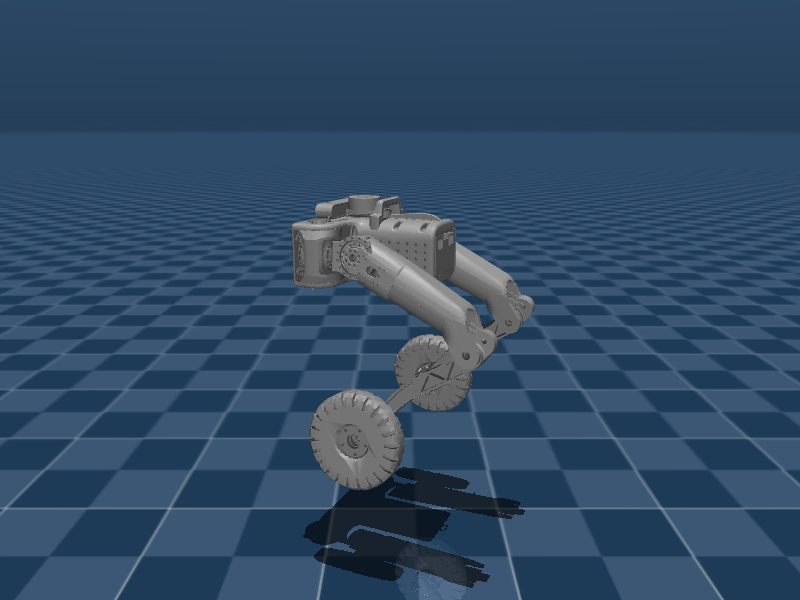
\includegraphics[width=0.32\columnwidth]{xqrobotwl_render.png}
    \caption{xqrobotwl 两轮足机器人}
    \label{fig:robot}
\end{figure}

\begin{table}[htbp]
    \centering
    \caption{xqrobotwl 主要参数}
    \label{tab:robot_params}
    \begin{tabular}{lcc}
        \toprule
        参数 & 值 & 说明 \\
        \midrule
        总质量 & 18.65\,\text{kg} & 基座+双肢+双轮 \\
        机身质量 & 5.41\,\text{kg} & 含电池/电路/外壳 \\
        车轮质量（单侧） & 2.32\,\text{kg} & 含轮毂/轮胎/电机转子 \\
        车轮半径 & 0.065\,\text{m} & 轮地速度匹配所用 \\
        大腿长 $L_1$ & 0.224\,\text{m} & 髋—膝关节轴线距 \\
        小腿长 $L_2$ & 0.200\,\text{m} & 膝—轮心轴线距 \\
        单腿自由度 & 3+1 & 3旋转关节+1主动轮 \\
        控制频率 & 100\,\text{Hz} & $dt=0.01$\,s \\
        \bottomrule
    \end{tabular}
\end{table}

\subsection{与物理状态一致的相位门控奖励}

跳跃的难点在于时序：下蹲太浅则蹬伸无力，蹬伸过早则会与下蹲前馈相互抵消，落地速度过大则容易倾倒。为此，本文不仅使用跳跃指令计时，还将蹬伸类奖励与FSM的物理状态$s_t$绑定（表~\ref{tab:phase_reward}）。总奖励为
\begin{equation}
r_t = \underbrace{r_{\mathrm{base}}}_{\text{姿态、速度与对称性}} + \underbrace{\sum_i \mathbb{1}[s_t\in\mathcal{S}_i]\,r_i}_{\text{FSM状态门控项}},
\label{eq:reward}
\end{equation}
其中$r_{\mathrm{base}}$为存活、姿态、速度追踪、双腿对称与动作平滑等基础项，$\mathcal{S}_i$表示奖励$r_i$允许激活的FSM状态集合。

\begin{table}[htbp]
    \centering
    \caption{相位门控的跳跃奖励项（关键项）}
    \label{tab:phase_reward}
    \begin{tabular}{llp{6.5cm}}
        \toprule
        奖励项 & 相位区间 & 作用 \\
        \midrule
        crouch\_prep / crouch\_depth & $p\in[1,18]$ & 下蹲蓄力：机身降至下蹲目标，姿态前倾、屈膝、髋不外展 \\
        vertical\_thrust & $s_t\ge1$ 且$v_z>0$ & 仅在蹬伸及后续状态奖励竖直速度，禁止下蹲相提前上升 \\
        jump\_height & $p\ge1$ & 腾空高度：双轮离地且膝不锁死时按高度给奖 \\
        wheel\_air\_time & $p\ge1$ & 腾空奖励+空中轮空转惩罚 \\
        height\_progress & $s_t\ge1$ & 仅在蹬伸及后续状态奖励新的回合最高点 \\
        landing\_soft & 真实腾空落地段 & 软着陆：按$\exp(-|v_z|/0.5)$对落地速度缓冲；PPO系以“腾空后着地”计时器门控，杜绝站桩白嫖 \\
        lean\_forward & $j_{cmd}\le0.5$ & 站姿防后仰：站立期罚后仰与伸腿 \\
        \bottomrule
    \end{tabular}
\end{table}

对于无FSM的PPO消融，无法使用$s_t$门控，因此将蹬伸代理量改为窗口内的\textbf{实际升高}（launch\_rise），即
\begin{equation}
r_{\text{launch}} = \text{clip}(z_{\text{base}} - z_{\min}^{\text{window}},\, 0,\, 1) \cdot \mathbb{1}[\text{着地}\wedge\text{已下蹲}],
\label{eq:launch_rise}
\end{equation}
式中$z_{\min}^{\text{window}}$为当前触发窗口内机体最低高度。对SRL+VMC而言，$s_t\ge1$的物理门控是更关键的一步：修改前，策略可在下蹲状态先用腿长残差把机体顶起，随后被FSM下蹲参考拉回，最后再真正起跳。关闭下蹲相的vertical\_thrust和height\_progress后，这一奖励漏洞被消除。

\subsection{SLIP-FSM 相位参考}

借鉴SLIP模型“储能—释能”的相位划分，本文用六状态有限状态机（FSM）为跳跃周期提供结构化时序参考（表~\ref{tab:fsm}）。与点足跳跃框架不同，两轮足的飞行阶段并非纯弹道：飞行中需保持收腿姿态，并在落地前将轮速同步至地面速度，故状态2（腾空）与状态3（落地准备）均含明确的车轮行为。

\begin{table}[htbp]
    \centering
    \caption{面向两轮足跳跃的六状态有限状态机}
    \label{tab:fsm}
    \begin{tabular}{clll}
        \toprule
        状态 & 名称 & 腿部参考 & 车轮行为 \\
        \midrule
        -1 & 待机 & 默认站姿 & 静止 \\
        0 & 下蹲 & 屈膝下蹲 & 制动/低扭矩稳定 \\
        1 & 蹬伸 & 腿部爆发伸展 & 主动驱动提供额外冲量 \\
        2 & 腾空 & 收腿保持 & 轮速斜坡同步地面速度 \\
        3 & 落地准备 & 缓冲力减速 & 轮速同步地面速度 \\
        4 & 恢复 & 恢复站姿 & 过渡至倒立摆平衡 \\
        \bottomrule
    \end{tabular}
\end{table}

状态转换由传感器信号驱动：待机$\to$下蹲触发跳跃指令（$j_{cmd}>0.5$且驻留$>0.1$\,s）；下蹲$\to$蹬伸驻留超过$t_{\text{crouch}}$（关节空间$0.25$\,s，VMC$0.35$\,s）；蹬伸$\to$腾空驻留超过$t_{\text{thrust}}$（关节空间$0.20$\,s，VMC$0.30$\,s）；腾空$\to$落地准备为竖直速度转负且高度接近地面；落地准备$\to$恢复为机身高接近地面且缓冲驻留$>0.05$\,s；恢复$\to$待机驻留$>0.15$\,s。FSM输出逐状态的参考：关节空间变体为6维关节角参考$ \bm{a}_{\text{ff}}$，VMC变体为虚拟腿长参考$L_0^{\text{ref}}$（下蹲$0.28$\,m、蹬伸$0.50$\,m、腾空收腿$0.26$\,m、落地$0.30$--$0.42$\,m）。策略输出与参考按反馈增益融合：
\begin{equation}
\bm{u}_t = \bm{u}_{\mathrm{FSM}}(s_t) + g\,\Delta\bm{u}_{\pi}(o_t,s_t),
\label{eq:action}
\end{equation}
其中$\bm{u}_{\mathrm{FSM}}$是虚拟腿长、腿角和轮速参考，$\Delta\bm{u}_{\pi}$是策略残差，$g=0.5$限制策略对结构化参考的覆盖程度。FSM状态与计时器作为额外观测拼接进策略输入，使策略可依据当前相位学习不同的残差修正。

\subsection{虚拟模型控制（VMC）层}

VMC（虚拟模型控制~\cite{pratt2001vmc}）将策略输出从关节空间映射到\textbf{虚拟腿坐标}，再经雅可比反解为关节力矩。每条腿定义腿角$\theta_0$（矢状面内相对竖直方向）与腿长$L_0$（髋至轮心），其正运动学为
\begin{equation}
L_0 = \sqrt{x_{\text{end}}^2 + y_{\text{end}}^2},\qquad
\theta_0 = \mathrm{arctan2}(y_{\text{end}}, x_{\text{end}}) - \frac{\pi}{2},
\label{eq:fk}
\end{equation}
其中$x_{\text{end}}, y_{\text{end}}$为髋坐标系下轮心的解析位置。由于xqrobotwl的关节轴与参考机器人不同（膝关节在$q_{\text{knee}}=0$时已弯曲约$96^\circ$，腿无法完全伸直），腿长与腿角的符号约定经数值标定拟合（$l_1=0.3005$\,m，$l_2=0.3007$\,m，双腿正解RMSE$<3$\,mm）。控制律为
\begin{align}
\tau_{\theta_0} &= k_{p,\theta}(\theta_0^{\text{ref}}-\theta_0) - k_{d,\theta}\dot\theta_0,\\
F_{L_0} &= k_{p,L}(L_0^{\text{ref}}-L_0) - k_{d,L}\dot L_0 + F_{\text{ff}},
\label{eq:vmc_law}
\end{align}
式中$F_{\text{ff}}=110$\,N为每腿支撑前馈力（机器人每腿承重约91\,N），保证静态支撑。$(\tau_{\theta_0}, F_{L_0})$经2连杆雅可比映射为髋、膝力矩，髋滚转用PD控制、轮速用PI控制。VMC参数随FSM相位动态调整：蹬伸阶段刚度与前馈放大3倍、阻尼降为1/4以爆发蹬地，落地阶段阻尼放大2.5倍以缓冲。该设计使策略能以力矩级控制爆发式蹬伸，同时保持柔顺缓冲。

\subsection{网络与训练设置}

四个变体共用PPO骨架~\cite{schulman2017ppo}：Actor与Critic均为4层全连接网络$[512,512,256,128]$（ELU激活），输出8维动作。观测由9帧历史本体状态拼接而成；SRL与最终SRL+VMC均拼接FSM状态与计时器，使用$315$维观测，以避免将额外虚拟腿观测与VMC执行层的效果混淆。关键超参为：学习率$1\times10^{-4}$，熵系数$0.005$，裁剪阈值$0.2$，折扣因子$0.99$，GAE $\lambda=0.95$，批大小$1024\times24$，训练10000轮。最终SRL+VMC训练累计产生$2.4576\times10^8$个环境步，单张RTX~4090上用时约1.82\,h。

\section{实验}

\subsection{训练与评估协议}

四个变体均在MuJoCo中使用1024个并行环境训练，每轮每环境收集24步。主方法SRL+VMC报告10000轮最终检查点，不根据评估结果挑选早期模型。评估使用策略分布的均值动作，且不向控制器注入额外扶正力或确定性轨迹。除单次完整阶段检查外，对最终策略连续触发20次跳跃，统计真实腾空和落地恢复。评估指标定义如下：
\begin{itemize}
    \item \textbf{跳高}：$h_{\mathrm{jump}}=\max_tz(t)-z_{\mathrm{stand}}$，其中$z_{\mathrm{stand}}$为触发前稳定站立高度；
    \item \textbf{真实腾空}：双轮同时离地且腾空持续时间超过阈值，排除接触检测抖动；
    \item \textbf{恢复成功}：真实腾空后重新着地，且在恢复窗口末满足机体高度、直立度和角速度条件，同时未触发终止；
    \item \textbf{阶段完整性}：分别检查站立、下蹲、蹬伸、腾空、落地、恢复和最终姿态七项条件。
\end{itemize}

\begin{figure*}[htbp]
    \centering
    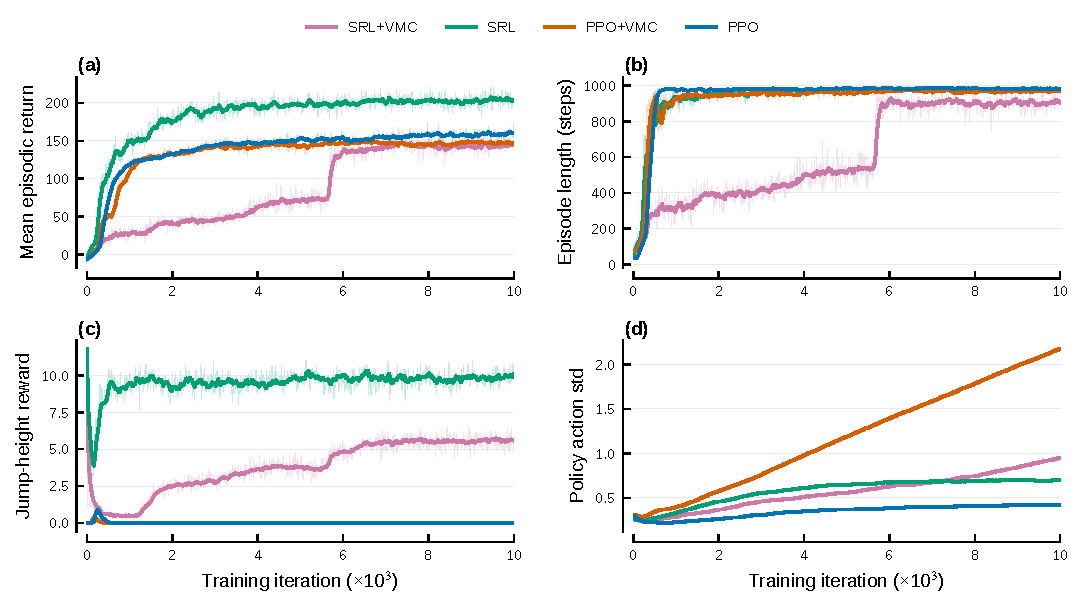
\includegraphics[width=0.94\textwidth]{fig_jump_flat_training_2x2_v3.pdf}
    \caption{四种组件组合在10000轮训练中的学习曲线。细线为原始记录，粗线为指数滑动平均；所有曲线均来自各方法最终模型对应的完整训练日志。}
    \label{fig:training}
\end{figure*}

\subsection{SRL+VMC完整方法结果}

最终SRL+VMC策略能够在跳跃指令前保持站立，指令触发后先将机体降至约0.315\,m，然后蹬伸进入腾空。当前最终检查点的完整阶段复测跳高为0.345\,m，腾空阶段直立度接近1.000，七项阶段与姿态检查全部通过。为降低单条轨迹偶然性，本文同时以20个独立复位回合报告均值与标准差，并以20次连续触发测试报告恢复成功率。

\begin{table}[htbp]
    \centering
    \caption{SRL+VMC最终策略的完整阶段评估}
    \label{tab:main_result}
    \begin{tabular}{lcc}
        \toprule
        指标 & 结果 & 判定 \\
        \midrule
        20回合平均跳高 & $0.308\pm0.006$\,m & 最高 \\
        完整阶段复测跳高 & 0.345\,m & 通过 \\
        腾空直立度 $u_z$ & 1.000 & 通过 \\
        完整阶段恢复 $|\omega|$ & 0.62\,rad/s & 通过 \\
        阶段/姿态条件 & 7/7 & 通过 \\
        20次连续触发 & 19次腾空，18次恢复 & 90\% \\
        \bottomrule
    \end{tabular}
\end{table}

20次连续触发中，19次形成真实腾空，18次在落地后恢复稳定站立，完整成功率为90\%。该协议下平均跳高为$0.346\pm0.069$\,m，最高为0.506\,m；一次尝试未形成有效腾空，另一次腾空后未恢复。结果表明完整阶段链已经形成，但高跳样本带来的落地冲击仍是主要失败来源。图~\ref{fig:trajectory}给出同一触发窗口内的代表性轨迹及本文方法的FSM相位。

\begin{figure*}[htbp]
    \centering
    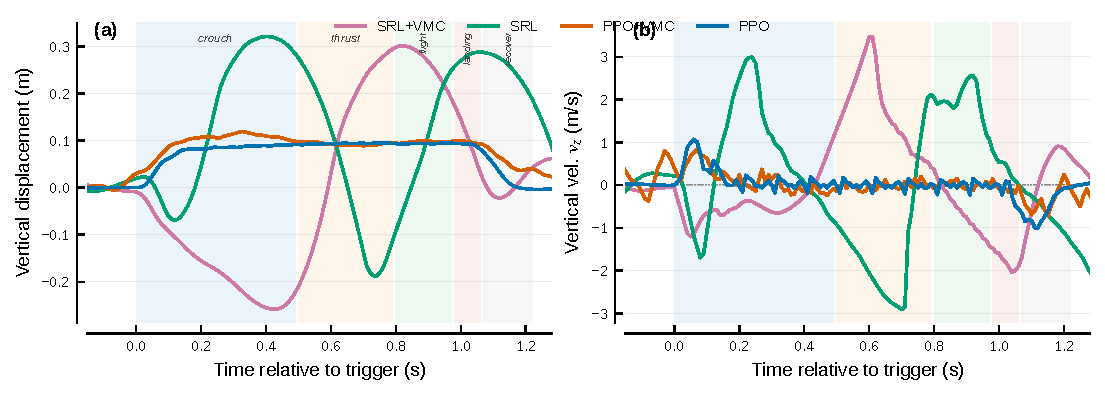
\includegraphics[width=0.94\textwidth]{fig_jump_flat_traj_2x1_v3.pdf}
    \caption{四种方法在单次触发窗口内相对于触发前站立高度的垂向位移和垂向速度。背景色表示SRL+VMC的下蹲、蹬伸、腾空、落地与恢复相位；终止后的仿真重置状态不计入轨迹。}
    \label{fig:trajectory}
\end{figure*}

\subsection{组件消融}

表~\ref{tab:ablation}给出四个最终模型各20个独立回合的跳高统计。完整SRL+VMC取得$0.308\pm0.006$\,m，较去除VMC的SRL提高23.0\%，较去除SLIP-FSM的PPO+VMC提高219.0\%。两个不含SLIP-FSM的变体均低于0.11\,m，说明对“先蹲后蹬”这类强时序动作，只靠奖励探索难以稳定形成足够的蓄力深度。图~\ref{fig:final_perf}进一步并列展示跳高与连续触发恢复率，完整方法的高度优势伴随10\%的恢复失败率，因此不能将高度优势等同于全面的鲁棒性优势。

\begin{table}[htbp]
    \centering
    \caption{SRL+VMC组件消融的20回合跳高（均值$\pm$标准差）}
    \label{tab:ablation}
    \begin{tabular}{lccc}
        \toprule
        变体 & SLIP-FSM & VMC & 跳高(m) \\
        \midrule
        纯PPO & 否 & 否 & $0.098\pm0.001$ \\
        PPO+VMC & 否 & 是 & $0.097\pm0.009$ \\
        SRL & 是 & 否 & $0.250\pm0.005$ \\
        \textbf{SRL+VMC（本文）} & 是 & 是 & $\mathbf{0.308\pm0.006}$ \\
        \bottomrule
    \end{tabular}
\end{table}

\begin{figure}[htbp]
    \centering
    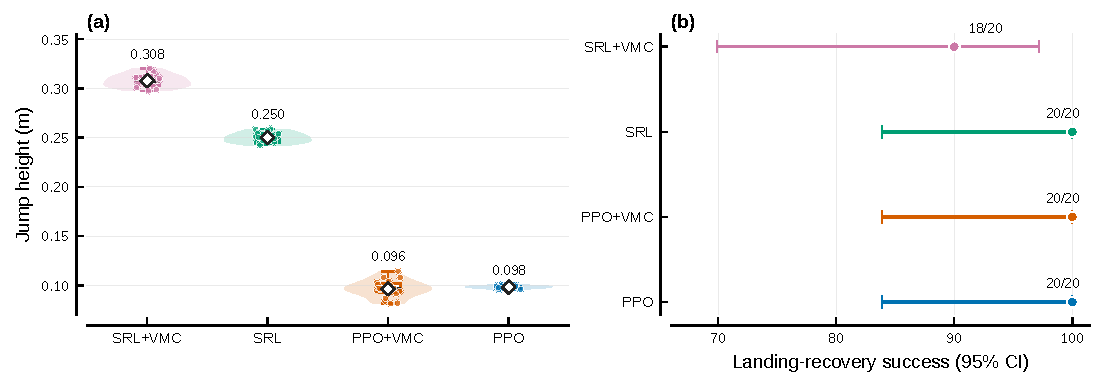
\includegraphics[width=\columnwidth]{fig_jump_flat_final_perf_2x1_v3.pdf}
    \caption{组件消融的最终性能。(a) 20个独立回合的跳高分布，散点为单回合数据，箱体表示四分位距，白色菱形表示均值；(b) 20次连续触发中的落地恢复成功率，误差线为二项分布Wilson 95\%置信区间。}
    \label{fig:final_perf}
\end{figure}

结果还表明，VMC不应被解释为对SLIP-FSM的替代。它为蹬伸与落地提供相位相关的柔顺性，但在无相位先验时仍不知道何时下蹲、何时释放能量。反之，SRL具有正确时序，但关节位置PD不能像VMC一样直接在虚拟腿空间调节蹬伸力与落地阻尼。

\subsection{FSM一致奖励门控的作用}

开发过程中，未将vertical\_thrust和height\_progress与FSM状态绑定的版本会形成“下蹲到位—提前升起—再次回落—真正起跳”的双重运动。其根因是下蹲状态的腿长残差上抬也能获得正奖励，与FSM的下蹲前馈构成相反目标。表~\ref{tab:gating}给出修改前后的评估结果。

\begin{table}[htbp]
    \centering
    \caption{FSM一致奖励门控前后的SRL+VMC性能}
    \label{tab:gating}
    \begin{tabular}{lcc}
        \toprule
        指标 & 未按FSM门控 & 按FSM门控（本文） \\
        \midrule
        轨迹形状 & 双重运动 & 单峰起跳 \\
        典型跳高 & $0.225\pm0.038$\,m & $0.308\pm0.006$\,m \\
        完整评估跳高 & $0.229$--$0.266$\,m & $0.345$\,m \\
        腾空直立度 & $0.992$--$0.996$ & $1.000$ \\
        恢复$|\omega|$ & $0.52$\,rad/s & $0.62$\,rad/s \\
        20次重复成功率 & $100\%$ & $90\%$ \\
        \bottomrule
    \end{tabular}
\end{table}

门控后策略下蹲更深，且在蹬伸状态中将动量集中到一次起跳，因此轨迹更干净、跳高更大。但跳高增加也带来更大落地冲击，使重复成功率从开发版本记录的100\%降至当前复测的90\%。由于两列来自不同开发检查点，该表用于解释设计演化而非严格配对统计；它说明奖励门控解决了轨迹时序问题，但高跳的落地鲁棒性仍需单独处理。

\section{讨论}

实验支持本文的核心判断：对两轮足跳跃，SLIP-FSM与VMC不是互相排斥的两种控制方案，而是分别解决“何时做什么”和“如何以合适的力去做”的两个层次。残差强化学习则连接了理想化参考与非线性轮腿动力学。这一结构与Hu等~\cite{hu2026srl}的模型先验和策略残差思路一致，但通过虚拟腿力控、相位变刚度/阻尼和轮速匹配扩展到了滚动接触平台。

同时，结果显示高跳与稳定落地之间存在明显张力。奖励门控使动量释放更集中，但这也将落地冲击推向了当前VMC和策略的鲁棒性边界。因此，90\%的重复成功率不应被表述为已完全解决跳跃问题，而是说明完整阶段链已形成，落地鲁棒性仍是主要瓶颈。

\textbf{局限与边界。}本研究存在以下限制：(1)结果全部来自MuJoCo仿真，尚未验证执行器延时、峰值电流和轮地摩擦误差下的实物性能；(2)每种方法仅训练一个随机种子，20回合评估只能反映回合级波动，不能替代多训练种子的统计显著性检验；(3)组件消融中与控制表达相关的观测和奖励做了必要适配，不是只替换一行控制器代码的严格正交实验；(4)尚未评估地面摩擦、质量、腿长和通信延时随机化下的鲁棒性。

\section{结论}

本文提出了一种面向两轮足机器人的SRL+VMC跳跃方法。该方法用SLIP-FSM规定下蹲、蹬伸、腾空、落地和恢复的相位结构，用PPO学习虚拟腿目标的残差，再由相位自适应VMC实现柔顺力矩控制。与FSM物理状态一致的蹬伸奖励门控消除了下蹲相提前上升导致的双重运动。最终策略在20个独立回合中取得$0.308\pm0.006$\,m的平均跳高，完整阶段复测达到0.345\,m并通过七项检查；20次连续触发中18次完成落地恢复。组件消融说明SLIP-FSM与VMC分别负责时序结构和柔顺力控，两者与残差学习结合后取得最高平均跳高。后续工作将通过多随机种子、域随机化和实物试验重点提升高跳落地的鲁棒性。

% ==================== 参考文献 ====================
\printbibliography[title={参考文献}]

\end{document}
